\section{Fundamentação teórica}
\subsection{Democracia e Sistemas Eleitorais Democráticos}
Diversas formas de governo se estabeleceram ao longo dos séculos, 
as primeiras formas que se tem indicio foram elaboradas por Aristóteles discípulo
de Platão, posteriormente outros pensadores como Maquiavel e Montesquieu se propuseram
à pensar as formas de governo, e até certo ponto chegaram a pensamentos conclusivos semelhantes.
Montesquieu menciona a democracia como uma fundamental forma de governo e à relaciona
com a república. 
Para Montesquieu, “quando, em uma republica, o povo como um todo possui o poder soberano,
trata-se de uma democracia”. \cite{de1857oeuvres}. Com isso, podem-se perceber 
claramente que para que haja uma sociedade democrática, a população deve exercer
o poder sobre o Estado. \par
Como bem se sabe a palavra democracia é oriunda do Grego \emph{(demos, povo; kratos, poder)} 
que significa \emph{poder do povo}. Baseado no conceito fundamental da democracia
pode-se estar governando uma só pessoa ou um grupo de representantes, desde que
a escolha destes indivíduos seja realmente do povo é considerado uma forma de governo
democrático \cite[A democracia]{ribeiro2001democracia}. \par 
A principal referência que tem-se em democracia com toda certeza foi o regime de Atenas, 
o próprio povo ou a própria nação, composta dos cidadãos que à formavam,
decidia em praça pública seus problemas fundamentais, com base nisto é razoável
imaginar que não era um modelo escalável, ou seja, conforme a população se tornava 
mais numerosa, mais complicada tornavam-se as reuniões em praças públicas. 
Calcula-se que o número de cidadãos, que decidiam os assuntos do Estado,
não ia muito adiante de 40.000, embora nas assembleias não comparecessem mais de
alguns milhares de cidadãos. Não se poderia pensar em democracia direta com os
Estados modernos, seu território e a população de cada um deles. 
Daí a necessidade de um regime, que dispensasse a presença da totalidade dos 
cidadãos, sem eliminar o direito de pronunciamento de cada um deles. 
Para chegar a esse resultado é que se foi imposto o Regime Representativo democrático,
em que o cidadão elege os governantes e estes decidem em seu nome ou em seu lugar.
Foi uma fórmula prática para a solução do problema. quando se entendeu que era
preciso convocar o povo, para que o governo se exercesse em seu nome e, 
de alguma forma, com a sua responsabilidade ou a sua intervenção.
\cite[Eleição e Sistemas Eleitorais]{sobrinho1958eleiccao}. \par
A democracia está quase sempre presente nas falas dos principais
líderes dos mais diversos países, sua importância na consagração da legitimidade
dos governantes, faz com que mesmo regimes não democráticos recorram a processos
eleitorais, buscando trazer para o regime apoio popular.\par
\begin{quote}
"Parodiando La Rochefoucauld, poderíamos dizer que este uso das eleições, nos 
regimes ditatoriais, constitui uma homenagem que os governos não democráticos
rendem aos princípios cardeais da democracia". \cite[Eleição e Sistemas Eleitorais]{sobrinho1958eleiccao}.
\end{quote} \par
Leva-se a conclusão de que apenas uma eleição não garante a existência de um
regime democrático. É preciso também que a eleição seja realizada dentro de um 
rigoroso processo com determinadas garantias que assegurem a liberdade do voto
e a autenticidade das apurações; daí, também, a atenção que essas técnicas têm
merecido, no estudo e aplicação das leis, que organizam e disciplinam os sistemas eleitorais. \par
Existem inúmeras formas de classificar os sistemas eleitorais, neste documento nôs atentaremos
ao sistemas democráticos. De acordo com Jairo Nicolal cientista político brasileiro
e especialista em sistemas eleitorais em seu livro "Sistemas Eleitorais" \cite{nicolau2015sistemas}
baseado nas obras de alguns estudiosos \cite{blais1997electoral},
pode-se caracterizar os mais diversos sistemas eleitorais democráticos em todo o mundo,
em três grupos: os majoritários, os proporcionais e os mistos. Cada qual com 
seus respectivos sistemas.

\begin{figure}[htb]
	\caption{\label{exemplo}Sistemas Eleitorais Democráticos}
	\begin{center}
	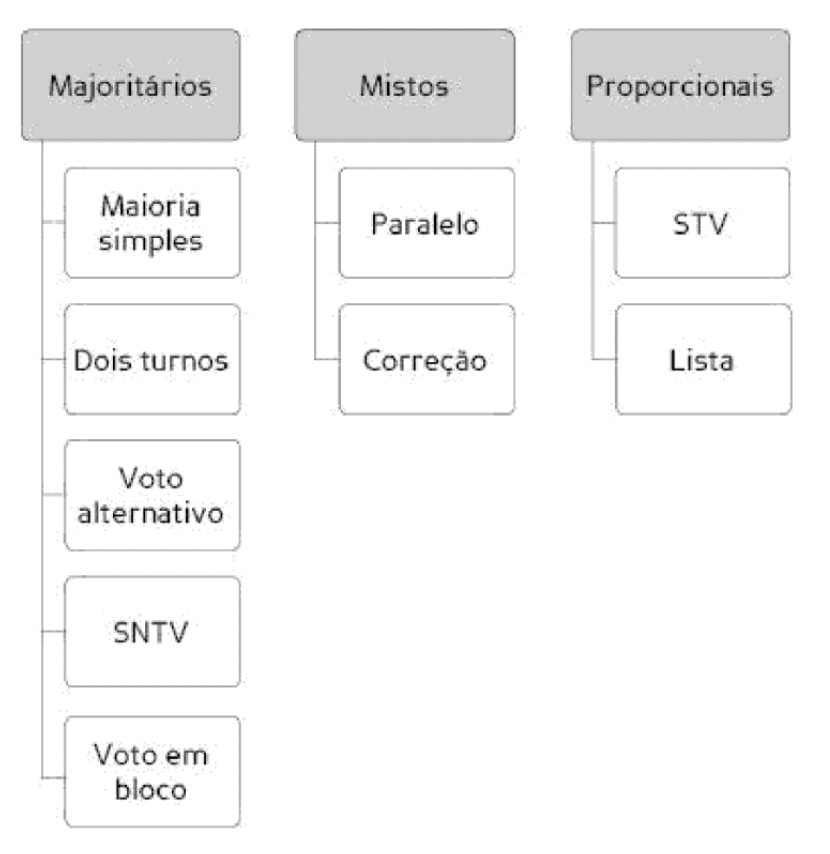
\includegraphics[scale=0.7]{textual/sistemas-eleitorais.png}
	\end{center}
	\legend{Fonte: Sistemas eleitorais \cite{nicolau2015sistemas}}
\end{figure} 
\subsubsection{Sistemas Eleitorais Majoritários}
O sistema majoritário é um dos principais meios de escolha de representantes em 
democracias representativas. Em suma ocorre um sistema de votação direta onde o
candidato mais votado recebe 100\% da representação. Os demais partidos ficam sem
representação. Há variações deste modelo com a possibilidade de implantar ou não 
um contingente mínimo de votos para que o candidato mais votado seja eleito. Contudo
apenas o sistema de maioria simples não garante que o candidato mais votado 
receba apoio de mais da metade dos eleitores, portanto para sanar esta condição
é estabelecida votações de dois turnos, onde dois
candidatos mais votados fazem uma nova eleição para então estabelecer por maioria
simples o vencedor. \cite[pág. 8]{nicolau2015sistemas}. Vale destacar que o voto por maioria
simples pode ser implementado por numero de eleitores ou por voto distrital, onde
vence o candidato com maior numero simples de distritos ou estados que o apoiam,
como é o exemplo das eleições do Canadá. Outra forma de complementar o sistema 
majoritário e evitar o problema gerado pela maioria simples, é o voto alternativo,
onde o eleitor vota em todos os candidatos adicionando uma ordem onde o primeiro 
colocado é sua principal opção e o ultimo sua opção alternativa. 
O candidato que recebe a maior preferência é eleito.\cite[pág. 7 - 16]{nicolau2015sistemas}.
\subsubsection{Sistemas Eleitorais Proporcionais}
Os sistemas proporcionais buscam um equilíbrio matemático entre os partidos
que disputam as eleições e a quantidade de cadeiras disponíveis para representação
dos eleitores. A quantidade é distribuída de acordo com a proporção de votos de
cada partido. Em tese esta abordagem assegura que a adversidade de opiniões
de uma sociedade esteja totalmente refletida no Legislativo. Dentro do sistema
proporcional há ainda duas variantes possíveis: o voto único intransferível e o
sistema de listas, o primeiro caso estabelece uma quota de votos, afim de garantir
que cada candidato esteja apto a representar já que sua representação seria considerada
relevante, já o segundo a quota é estabelecida da mesma forma, porém com o partido.
\cite[pág. 29]{nicolau2015sistemas}.
\subsubsection{Sistemas Eleitorais Mistos}
Os sistemas mistos são os processos eleitorais que envolvem ambos os sistemas 
majoritários e proporcionais para decisões de representantes em um mesmo cargo.
Se por um lado é estabelecido quotas para ocupação através de voto único transferível
ou lista, por outro essa ocupação é definida baseando-se em uma maioria que pode
ser estabelecida por voto distrital, dois turnos, voto alternativo, por maioria 
simples etc. Até o final dos anos de 1980 apenas o México e a Alemanha utilizavam
sistemas eleitorais mistos.\par 
É válido destacar que para análise dos grupos citados anteriormente,
é levado em conta um relatório produzido pela organização americana Freedom House,
que avalia o grau de democracia anualmente em vários países, levando em consideração
uma série de aspectos, entre eles considera-se principalmente se há eleições 
livres e limpas.\cite{puddington2011freedom}. \par
Independente do sistema adotado, com base nos sistemas democráticos apresentados
pode-se afirmar que para ser considerado um sistema eleitoral democrático de direito
é necessário que o sistema atenda a quatro premissas:
\begin{itemize}
  \item O sistema deve especificar um meio para que o desejo de voto seja computado;
  \item O sistema deve deixar claro o conjunto de votos permitidos;
  \item O sistema deve conter um método de contabilizar os votos;
  \item O sistema deve estabelecer um algoritmo que determine o resultado da eleição.
\end{itemize} \par
Afim de esclarecer, não é o propósito deste documento avaliar qual o melhor 
sistema eleitoral, mas sim afirmar que independente 
do sistema adotado ambos possuem como objetivo final garantir a representação
democrática através da legitimidade do voto. Considerando este aspecto e 
o que as eleições significam é necessário reconhecer a importância que 
o processo eleitoral possui.
\begin{quote}
Já lembrava Montesquieu: "As leis que estabelecem o direito de voto são, pois,
fundamentais nesse governo. Realmente, é tão importante regular como. por quem, 
a quem, sobre que devem ser dados os sufrágios, quanto saber, na monarquia, 
quem é o monarca e de que maneira deve governar. Libânio diz que "em Atenas um 
estrangeiro que se misturasse na assembleia do povo era punido com a morte.
É que esse indivíduo usurpava o direito de soberania". Acrescentava Montesquieu
que a lei. que regulava a maneira de votar, numa democracia, não podia deixar 
de ser considerada como uma lei fundamental. \cite[Pág. 173]{sobrinho1958eleiccao}.
\end{quote}\par
Com base nas falas de Montesquieu e Libânio, é sensato dizer que a falta de confiança
em sistemas eleitorais e na legitimidade do voto, pode corromper profundamente
o significado da democracia representativa ou participativa. Já que a fraude 
ou corrupção nas eleições levariam à eleição de representantes ilegítimos, 
ou seja, que não estão de acordo com a vontade e soberania do povo gerando
retrocesso nos direitos sociais, regimes autoritários e totalitários, 
impeachments e até mesmo desestabilização econômica.\par


\clearpage